\documentclass[a4paper,11pt]{article}
\usepackage[utf8]{inputenc} %% pues [utf8x] da problemas
\usepackage{amsmath,amsfonts,amssymb}
\usepackage{alltt}
\usepackage[]{fancyhdr}
\usepackage{latexsym}
\usepackage{graphicx}
\usepackage{subfigure}
\usepackage{makeidx,epsf}
\usepackage[colorlinks,bookmarksopen,bookmarksnumbered,citecolor=blue,urlcolor=red,colorlinks=true,linkcolor=blue]{hyperref}
\usepackage{nameref,url}
\usepackage{subfigure}
\usepackage[T1]{fontenc}
\usepackage[spanish]{babel}
\usepackage[colorinlistoftodos]{todonotes}
\usepackage{setspace}
% ...........................................................
\usepackage{paralist}   % para {compactitem}
\usepackage{enumitem}   % para {itemize}[noitemsep]
\usepackage{sistyle}    % an intermediate SI units package 
%usepackage{siunitx}    % better SI units that collects several ones
% .........................................................
% .........................................................
%\usepackage{bibunits}
\usepackage[babel]{csquotes}
\usepackage{soulutf8}
\usepackage{multicol}
% ..............................................................
%\usepackage[hyperref,backend=biber,natbib=true]{biblatex}
%% \addbibresource{sloshing3d.bib}
%% \addbibresource{navales.bib}
% --------------------------------------------------------------
\newcommand{\avv}{\langle\mathbf{v}\rangle}
\newcommand{\avp}{\langle{p}\rangle}
\newcommand{\rearrow}[2]{\ensuremath{~~\substack{\xrightarrow[]{~#1~}\\\xleftarrow[~#2~]{}~~}}}
\scrollmode \makeindex \sloppy
\decimalpoint  % numeros decimales con punto
% ----------------------------------------------------------------
% macros usuario
% ----------------------------------------------------------------
% longitudes y centrado de la caja, espaciado:
  \textheight = 25.70 truecm
  \textwidth  = 17.50 truecm
  \advance\voffset by  -2.0 truecm     % \voffset = -1 truein
  \advance\hoffset by  -2.0 truecm     % \hoffset = -1 truein
  \renewcommand\baselinestretch {1.2}  % interline
% ----------------------------------------------------------------
% definiciones del usuario
\newcommand{\of}{OpenFOAM\textsuperscript\textregistered}
\newcommand{\ltitle}[1]{{\normalsize {\bf #1 }}}
\newcommand{\stitle}[1]{\begin{center} \normalsize \bf #1 \end{center}}
\catcode`\!=\active
\let!\boldmath
\def\!{\ifmmode\mskip-\thinmuskip\else\char'74\fi}
%
%% \let\oldbibliography\thebibliography
%% \renewcommand{\thebibliography}[1]{%
%%   \oldbibliography{#1}%
%%   \setlength{\itemsep}{1pt}%
\makeatletter
\renewenvironment{thebibliography}[1]
    {\begin{multicols}{2}[\section*{\refname}]%
      \@mkboth{\MakeUppercase\refname}{\MakeUppercase\refname}%
      \list{\@biblabel{\@arabic\c@enumiv}}%
          {\settowidth\labelwidth{\@biblabel{#1}}%
            \leftmargin\labelwidth
            \advance\leftmargin\labelsep
            \@openbib@code
            \usecounter{enumiv}%
            \let\p@enumiv\@empty
            \renewcommand\theenumiv{\@arabic\c@enumiv}}%
      \sloppy
      \clubpenalty4000
      \@clubpenalty \clubpenalty
      \widowpenalty4000%
      \sfcode`\.\@m}
     {\def\@noitemerr
       {\@latex@warning{Empty `thebibliography' environment}}%
      \endlist\end{multicols}}
\makeatother

% ----------------------------------------------------------------
\title{ DESCRIPCIÓN TÉCNICA - PICT 2021 \\ %% HASTA 20 PÁGINAS, 2MB
 {%\Large 
 Título:  \bf Métodos numéricos de alto desempeño en dinámica de fluidos computacional para problemas de interfases móviles}}
%%Desarrollo de métodos numéricos de alto desempeño para multifísica computacional:
%%     interfases, medios permeables  e interacción fluido-estructura.}}
%% PID UTN 2020 Métodos numéricos eficientes y escalables para el estudio de flujos y sus efectos en obras civiles
%% PIP 2021 Dinámica de fluidos computacional para flujo y transporte multifásico en plataformas de supercómputo
%% PICT 2018 Dinámica de fluidos computacional con aplicaciones en interfases móviles a diferentes escalas
%% PID UTN 2019 Prototipos numéricos de alto desempeño computacional para flujo y transporte multifásico enaplicaciones ingenieriles
\author{L. Battaglia, J. D'El\'{\i}a, L. Garelli, P.A. Kler (IR), G.A. R\'{\i}os Rodr\'{\i}guez y M.A. Storti.}
\date{}
% --------1--------------------------------------------------------
\begin{document}
%\pagenumbering{0}
\vspace{-1cm}
\maketitle
\if 0
\section*{Palabras clave y temas}

\begin{itemize}
\item Interacción fluido-estructura: energía undimotriz, fuerzas sobre cuerpos sumergidos.  
\item Interfases móviles: generación de microgotas, flujo multifase en medios permeables. 
\item Superficie libre: agitación, tanques de olas numéricos. 
\end{itemize}

\section*{Otros integrantes}

Posibles: EJ López, S Sarraf

\textcolor{red}{revisar: Marcela Cruchaga, Mandy, otros colaboradores }

Cuchu, Seba Toro, fede schaumburg, Guille castro, Camilo meyer, mariano rubiolo

Becarios: Gerlero, Arriondo, Harispe, Salazar, Caram, Franck, Trivisonno, Inzeo


\section*{Resumen}
Este proyecto se propone desarrollar técnicas de simulación numérica computacional en dinámica de fluidos para el adecuado estudio y desarrollo de aplicaciones tecnológicas que involucran interfases entre fluidos inmiscibles, pudiendo considerarse interfases
líquido-gas, líquido-líquido, o líquido-sólido abarcando diferentes escalas de longitud. Se considerará el estudio de las interfases mencionadas tanto en entornos abiertos como en el caso de cuerpos inmersos y flotantes, depósitos y canales de líquidos con superficie libre, como en entornos confinados como tubos o canales de diferentes dimensiones geométricas, y en medios porosos artificiales o naturales, como en el caso hormigones drenantes, suelos o medios de uso en microfluídica. 

Las aplicaciones en las que se enfoca fundamentalmente este proyecto se orientan al sector energético, a través de las aplicaciones en generación undimotriz, y al sector medioambiental tanto en el manejo optimizado del ciclo de aguas en zonas urbanas y estructuras civiles (a partir del desarrollo de diferentes elementos constructivos basados en hormigones drenantes), como en el monitoreo de contaminantes a través de herramientas microfluídicas.

Para el desarrollo de los algoritmos de simulación numérica propuestos, se utilizarán herramientas de código abierto basadas principalmente (aunque no exclusivamente) en el método de volúmenes finitos, las cuales se desarrollarán de acuerdo a las necesidades particulares de cada una de las aplicaciones. Todos los programas desarrollados se ejecutarán en plataformas de cálculo paralelo con alto desempeño computacional, principalmente en aquellas disponibles en el lugar de trabajo de los investigadores del proyecto.

\newpage
\fi
\section{OBJETIVOS GENERALES} 

%\begin{bibunit}[unsrt]

\if 0 {\it (máx 1 pág.)  Objetivos Generales e impacto: Identificar
  el problema general en estudio, contextualizar el problema a nivel
  local, identificar que parte del problema se intenta abordar  /contribuir con la investigación.}  \fi

El objetivo general de la propuesta es el desarrollo de métodos numéricos la resolución de problemas de interés tecnológico en el área
de la dinámica de fluidos computacional para modelar y representar fenómenos multifísicos que involucran interfases móviles de geometría fija y variable. Estos fenómenos requieren formulaciones
consistentes en la producción de estrategias numérico-computacionales
aptas para la verificación y diseño de sistemas y prototipos en 
diferentes escalas de interés, desde grandes estructuras para la generación de energía, o denajes urbanos, hasta aplicaciones en dispositivos portátiles de análisis en microfluídica.

Se promueve además que los métodos numéricos sean eficientes y escalables en un paradigma de computación paralela de alto desempeño, e
integrados a códigos de fuente abierta basados en métodos tales como el de volúmenes finitos, de elementos finitos y de elementos de borde, dando continuidad y proyección a futuro a los desarrollos del grupo de
trabajo tanto en los conocimientos básicos asociados a los métodos como en los desarrollos tecnológicos en las diferentes temáticas de las aplicaciones.

Desde el punto de vista de las aplicaciones, este proyecto busca desarrollar de manera más enfática las capacidades del grupo para intervenir en procesos innovativos en aplicaciones energéticas (a través de la generación undimotriz) y medioambientales (a través de la optimización de drenajes y saneamiento y control de aguas urbanas).

\textcolor{red}{Falta enfatizar lo novedoso, nuevos fenómenos a
  incorporar, mayor precisión o detalle, para diferenciarlo del
  PICT2018.  }

\newpage

\section{OBJETIVOS ESPECÍFICOS E HIPÓTESIS DE TRABAJO} 
%\iftrue
\if 0
{\it (máx 1 pág)
Identificar los Objetivos específicos relacionados con el problema que se abordará. Describir la hipótesis de trabajo y como se abordará el problema en cuestión a través de la experimentación y estudio.}
\fi

{Los objetivos específicos están orientados a desarrollar métodos numéricos} {para resolver problemas específicos de mecánica de fluidos  computacional donde las interfases juegan un rol preponderante en la estimación de parámetros y fenómenos de interés tecnológico. Además del desarrollo de los métodos, será crucial su implementación utilizando códigos y lenguajes específicos, de uso corriente por parte del grupo de trabajo, para su ejecución en infraestructuras de  computación de alto desempeño}. 
Los fluidos involucrados en los dominios de cálculo serán en general considerados incompresibles, invíscidos o viscosos, {mientras que los elementos sólidos serán considerados rígidos o elásticos con baja deformación}. 

%Los objetivos específicos del proyecto están dados en función de los fenómenos a resolver. 
%, brindando para cada uno el marco metodológico previsto.



%\textcolor{red}{Tomado de PIP 2021 derecho. Quizás haya que refrasear y meter hipótesis/abordaje. Tomo también la gente a trabajar, comentada dentro de cada subsection }

\paragraph{2.1 Interfases líquido--gas no confinadas: superficie libre.}
%Gustavo, Laura - ya refraseado
Generar algoritmos aptos y eficientes para resolver problemas de flujo a superficie libre, sea en recintos acotados -como los casos de agitación o {\it sloshing}- o en dominios con fronteras abiertas, tales que constituyen desafíos tanto en el conocimiento de la cinemática de la interfase como en los efectos dinámicos del fluido sobre los contornos o elementos interpuestos al flujo, como ser estructuras fijas o móviles sometidas a oleaje. La representación de la superficie libre en tres dimensiones espaciales será abordada mediante estrategias de captura de interfase desarrolladas sobre solvers basados principalmente en volúmenes finitos altamente escalables para flujo viscoso e incompresible.
\vspace{-0.2cm}
\paragraph{2.2 Interfases líquido--solido: interacción fluido-estructura.}
%Mario, Laura - ya refraseado 
Desarrollar métodos en volúmenes finitos con cuerpos embebidos incorporados mediante un término de penalidad en las ecuaciones de Navier-Stokes (NS) activado en la región ocupada por el sólido con el fin de resolver casos de interacción fluido-estructura, asumiendo cuerpos inmersos rígidos en flujo no estacionario, incompresible y viscoso, aplicable a cuerpos con movimientos impuestos -esto es, de trayectoria predefinida- o no restringidos, como en la sedimentación de partículas.  
%Gustavo, Jorge, Sofía?
\textcolor{red}{BEM para interacción fluido-MEMs?}
\vspace{-0.2cm}
\paragraph{ 2.3 Interfases líquido--gas confinadas: flujo en medios porosos en regimen saturado e insaturado.}\label{ss:oe21}
%Gabriel, Josy, Nico, Rodrigo, Pablo
Desarrollar técnicas y estrategias numéricas para la simulación de flujos capilares e hidrostáticos en medios porosos acoplando el transporte de solutos. El transporte de diferentes tipos de sustancias, consideradas como concentraciones escalares, se resolverá tanto en regímenes saturados como no-saturados para ambos tipos de flujo. Se considerarán diversos enfoques, algunos basados en simplificaciones tipo Washburn, otros basados en la ecuación de Richards con diferentes modelos capilares, y técnicas multiescala basadas en homogeneización. 
\vspace{-0.2cm}

\paragraph{2.4 Interfases líquido--sólido confinadas: flujo reactivo en  microestructuras}
%Joselynne, Seba, Camilo, Pablo
Desarrollar estrategias numéricas para la implementación de modelos reactivos en el estudio del comportamiento de reactores catalíticos microestructurados de interés medioambiental. Estas estrategias deben contemplar la naturaleza intrincada del flujo de fluidos a través de matrices de porosidad microestructurada (mencionada en el objetivo anterior) y las etapas fisicoquímicas que determinan los mecanismos reactivos como la difusión, la adsorción y la activación.
\vspace{-0.2cm}

\paragraph{2.5 Interfases líquido--líquido confinadas: flujo bifásico inmiscible en microgotas}
%David, Pablo y Jorge
Obtener implementaciones numéricas consistentes y eficientes para modelar los diferentes fenómenos que involucran la ruptura de interfases líquido-líquido, como la coalescencia y división de gotas. Se proponen tres estrategias diferentes con diferentes complejidades computacionales: modelos semi-empíricos, modelos completos \textit{Volume of Fluid.} (VOF) y modelos híbridos VOF--dos fluidos combinados con aprendizaje maquinal.

\newpage

\section{RELEVANCIA DEL PROBLEMA} 
\if 0
{\it (máx 3 pág.)
Desarrollar la importancia e impacto a nivel local, general y para la especialidad del problema, los objetivos y el conocimiento que se generará.
Describir antecedentes, avances y el estado del arte – búsqueda bibliográfica actualizada.}
\fi
\subsection{Relevancia e impacto en el medio}
Los métodos computacionales contemporáneos para la resolución de problemas de ingeniería constituyen una ventaja operativa para todos los actores sociales intervinientes en desarrollos tecnológicos novedosos. Las simulaciones numéricas permiten disminuir costos de diseño, aumentar la factibilidad de los desarrollos, y disminuir sensiblemente los tiempos de llegada al mercado y/o al campo de uso de los productos desarrollados. Los prototipos numéricos permiten acotar la cantidad de situaciones a modelar físicamente, y brindan, en todos los casos, información instantánea y puntual de todas las magnitudes físicas involucradas, ya sean medibles o no en los prototipos reales. Se listan a continuación posibles impactos en el sector académico y socioproductivo asociados a las diferentes lineas de trabajo propuestas:
\begin{itemize}

\item{\bf Interfases líquido--gas no confinadas: superficie libre.}
  La verificación y diseño de estructuras o componentes industriales en contacto con flujos a superficie libre requiere el conocimiento tanto de la posición de la interfase como de las características del escurrimiento y sus acciones hidrodinámicas, siendo los modelos computacionales una herramienta de consulta actual para el estudio de diferentes hipótesis y escenarios. Entre los casos de interés, se encuentran los de agitación de contenedores para almacenamiento o transporte de fluidos~\cite{Kamath2021sloshing,Jin2019}, los estudios de efectos dinámicos del oleaje sobre pilas de puentes, plataformas marinas o estructuras asociadas a generación de energía~\cite{Suja2018,Iuppa2019}.
  %% Calibracion de drag y demás, no me queda claro cómo lo hacen: https://www.sciencedirect.com/science/article/pii/S0029801822003250
  
\item{\bf Interfases líquido--solido: interacción fluido estructura. }
  A los ejemplos clásicos de interacción fluido estructura, tales como los de resistencia de olas en cascos de embarcaciones, se han sumado recientemente desarrollos tecnológicos en diferentes escalas, entre los cuales se cuentan sistemas micro-electromec\'anicos (MEMS)~\cite{Gesing2022} para aplicaciones específicas,  estructuras flotantes, como las dedicadas a acuicultura~\cite{Martin2022} o generadores de energía undimotriz o mareomotriz, entre ellos los dispositivos denominados \emph{Wave Energy Converters} (WEC) basados en la oscilación de un cuerpo o boya~\cite{Jin2022WEC}. 
  %% Effects of the end-stop mechanism on the nonlinear dynamics and power generation of a point absorber in regular waves // analitico https://doi.org/10.1016/j.oceaneng.2021.110123
  El acceso a modelos numéricos para estudiar los prototipos permite el análisis más detallado de los fenómenos que intervienen en el comportamiento de los componentes, así como también colaboran con la reducción de tiempos de desarrollo de los productos~\cite{Windt2020}. 
  
%% %

  
\item{\bf Interfases líquido--gas confinadas: flujo en medios porosos en regimen saturado e insaturado}
En los últimos años, muchas ciudades del litoral central argentino vienen incorporando sistemáticamente diversas políticas de manejo de aguas pluviales a los fines de mejorar la sustentabilidad y la seguridad hídrica de los cascos urbanos~\cite{ordenanza}. En este escenario, el hormigón permeable aparece como un elemento constructivo clave para la implementación exitosa de estas políticas. Sin embargo, al presente, son escasos los estudios de caracterización y modelos numéricos consistentes que permitan el diseño y la optimización de diferentes elementos constructivos basados en estos materiales~\cite{Pieralisi2017}. Paralelamente, los dispositivos basados en papel han demostrado un gran potencial para el desarrollo de diversas aplicaciones analíticas en salud, control ambiental, fitosanitario y bromatológico~\cite{Posthuma09,Yager06}. Al igual que en todos los casos anteriores, poder contar con herramientas de prototipado numérico que asistan al sector socioproductivo en los procesos de I+D, resulta de un impacto sustantivo. 


\item{\bf Interfases líquido--sólido confinadas: flujo reactivo en reactores microestructurados}
Una de las posibilidades que brindan los hormigones drenantes, y los materiales porosos en general, es el de aumentar sensiblemente las relaciones área--volumen. Este aumento, tiene su correlato de uso práctico en el aumento de la áreas de contacto fluido--sólido permitiendo incrementar la eficiencia de reacciones químicas catalizadas en superficie~\cite{xie2019permeable}. Durante su proceso de fabricación, los hormigones drenantes pueden funcionalizarse con diferentes tipos de catalizadores a los fines de pre-tratar o sanear parcialmente aguas urbanas. El impacto medioambiental de este tipo de tecnologías se presenta como relevante para todas aquellas políticas de manejo hídrico urbano por parte de los diferentes actores involucrados~\cite{mcintyre2021immobilization}.

\item{\bf Interfases líquido--líquido confinadas: flujo bifásico inmiscible en generadores de microgotas}
Se destacan notablemente en el campo de las aplicaciones contemporáneas de la microfluídica implementaciones de  microreactores~\cite{sui2020continuous}, microcápsulas multicapa para liberación controlada de drogas~\cite{Marengo2019generation}, microcámaras para cultivo de microorganismos~\cite{jian2020microbial}, entre otras otras~\cite{wang2019microdroplets}. 
En este contexto, para el desarrollo de estos dispositivos adquiere notoria importancia el empleo de prototipos numéricos que contribuyen a acelerar los procesos de diseño, ya que evitan iteraciones empíricas sobre prototipos reales~\cite{schaumburg_numerical}, con altos costos de mano de obra calificada, materiales, manufactura, e incluso ambientales. Sin embargo, los costos de las técnicas del estado del arte, en cuanto a la simulación numérica de flujo bifásico incompresible, son todavía incompatibles con los tiempos requeridos por la cadena de desarrollo de estos dispositivos.

%figuras PICT 2018
\if 0

%%%%%%%%%%%%%%%%%%%%%%%%%%%%%%%%%%%%%%%%%%%%%%%%%%%%%%%%%%%%%%%%%%
\begin{figure}[b]
\centerline{
  \includegraphics[width=3.6truecm]{./FIG/chueco-120h-bh-ta-co}
  \hspace{12pt}
  \includegraphics[width=3.6truecm]{./FIG/sculpt-120h-bh-ta-co}
  \hspace{12pt}
  \includegraphics[width=3.6truecm]{./FIG/squakn-4-3-0-bh-ta-co}
}% end centerline
\caption{\footnotesize 
  Flujo reptante por BEM/GBEM \cite{rf:jdelia-gbem3, rf:jdelia-gbem2} y 
  HBEM \cite{rf:ssarraf-hbem} alrededor de 
  geometr\'{\i}as intrincadas: 
  {\it hollow cube}     (izq.),
  {\it sculpted sphere} (cen.) y
  {\it square knots}  (der.), % \cite{rf:edelsbrunner1},
  generadas con \htmladdnormallink{NETGEN}%
  {http://sourceforge.net/projects/netgen-mesher},
  tracci\'on $\tau_1$ bajo flujo paralelo.} 
\label{fg-intrincate1}
\end{figure}
%%%%%%%%%%%%%%%%%%%%%%%%%%%%%%%%%%%%%%%%%%%%%%%
%%%%%%%%%%%%%%%%%%%%%%%%%%%%%%%%%%%%%%%%%%%%%%%
\begin{figure}[b]
\centerline{
\includegraphics[width=5.2truecm]{./FIG/ra75-17686-dg-ta-cw-4}
\hspace{10pt}
\includegraphics[width=6.2truecm]{./FIG/waves40}
}% end centerline
\caption{\footnotesize 
  GBEM: tracci\'on $t_x$ sobre una 
  micro-viga de polisilicio, perforada, doblemente empotrada, dimensiones $300 \times 100 \times {10}{\mu m}$, con $5 \times 15$ perforaciones de radio $r =  {4} {\mu m}$, y huelgo entre micro-viga y sustrato de $h = {4} {\mu m}$ (izq.)~\cite{rf:jdelia-gbem3}.
  %
  BEM: patr\'on de olas 3D detr\'as de un ferry 15 esloras 
  aguas abajo a una velocidad de 40 nudos (der.). 
 }
\label{fg-waves40}
\end{figure}
%%%%%%%%%%%%%%%%%%%%%%%%%%%%%%%%%%%%%%%%%%%%%%%%%%%%%%%%%%%%%%%%%%

%%%%%%%%%%%%%%%%%%%%%%%%%%%%%%%%%%%%%%%%%%%%%%%
\begin{figure}[tb]
\centerline{
\includegraphics[width=4.9truecm]{./FIG/boya1}
\hspace{10pt}
\includegraphics[width=5truecm]{./FIG/wec_usach_1.png}
}% end centerline
\caption{\footnotesize 
  Esquema de instalación de un dispositivo para generación de energía mareomotriz (izq.)~\cite{Falnes2007}.
  %
Prototipo para generación de energía undimotriz, gentileza USACH (der.). 
 }
\label{fg-boyas}
\end{figure}
%%%%%%%%%%%%%%%%%%%%%%%%%%%%%%%%%%%%%%%%%%%%%%%%%%%%%%%%%%%%%%%%%%
\fi
\end{itemize}

Las herramientas computacionales de código abierto involucradas en el proyecto resultarán aptas para su empleo en aplicaciones ingenieriles diversas, como las mencionadas, tanto por parte de actores privados como del Estado.  	
Estos prototipos numéricos permiten disminuir sensiblemente los costos por parte de emprendedores y PyMEs del ámbito regional y nacional durante las etapas de I+D y validación, como así también acelerar los procesos de introducción en el mercado de sus productos.
Asimismo, permitirán ampliar la capacidad de resolución de problemas en ámbitos académicos, tanto de investigación como de enseñanza en carreras de grado y de posgrado. La complejidad de las simulaciones que abarcan numerosos campos y escalas (multifísica) resultan sumamente demandantes en lo que refiere a la magnitud de los recursos computacionales necesarios para resolver con suficiente precisión cierto grupo de casos. Por este motivo, se trabajará a su vez en la resolución mediante herramientas de computación de alto desempeño en los clusters disponibles, tanto en la Unidad Ejecutora (UE) como en el Sistema Nacional de Computación de Alto Desempeño (http://www.supercalculo.mincyt.gob.ar). 
  


\subsection{Relevancia en la especialidad}

\textcolor{red}{ Faltan cosas de BEM. }

%% \subsection{Introducción general}
%% %2paginas
El modelado de interfases entre fluidos inmiscibles es un campo de investigación vigente y activo dentro de la disciplina de la mecánica computacional presentando desafíos en cuanto al modelado de los fenómenos, el comportamiento matemático de los modelos diferenciales propuestos, y el desempeño de las implementaciones computacionales de dichos modelos para las diferentes estructuras de cálculo disponible. Estos desafíos incluyen el desplazamiento de las interfases, la metodología empleada para identificar la posición de la interfase, el tratamiento numérico de la transición de las propiedades de los fluidos de un fluido al otro, el comportamiento elástico de las paredes sólidas, las condiciones de borde para dominios finitos o truncados y, en algunos casos, la representación de comportamientos reológicos diferentes en cada fase.



%Las ecuaciones de Navier-Stokes~\cite{rf:donea-huerta} para el caso incompresible y viscoso proveen el marco teórico para el cual se desarrollan los métodos numéricos que son de interés a este proyecto. Se agregan además todas las estrategias necesarias para que los modelos numéricos generados puedan resolverse en plataformas de cálculo distribuido de alto rendimiento (HPC).


%% El flujo a dos fases mediante simulación numérica ha sido abordado por métodos numéricos diversos~\cite{Cruchaga2016}, como por ejemplo diferencias finitas, volúmenes finitos, y elementos finitos, así como también métodos de partículas, en sus diversas variantes. Otro aspecto a destacar de la temática es la variedad de escalas geométricas que se incluyen en el estudio de interfases fluido-fluido~\cite{alkayyali2019microfluidic}. Estas escalas abarcan desde los cientos de metros, como en el caso del movimiento de olas, hasta algunas micras, como es el caso de las interfases capilares a nivel de poro en el papel~\cite{schaumburg2018numerical}. Otra circunstancia a tener en cuenta en el desarrollo de las técnicas numéricas son los efectos de la tensión superficial, en donde el cálculo preciso de las curvaturas juega un rol fundamental, sobre todo en interfases líquido--líquido~\cite{mora2019numerical}. Dada la variedad de temáticas y posibles enfoques, a continuación, se trata de compilar el estado del arte organizado de acuerdo a los diferentes tipos de aplicaciones contempladas en el proyecto.


%% \subsubsection{Intefases líquido-gas no confinadas: superficie libre}

%% El flujo con superficie libre se encuentra presente en diversos problemas de interés, como ser el escurrimiento en canales naturales o artificiales, en entornos marítimos en general~\cite{Yoshimura2019} y con aplicaciones a generación de energía~\cite{Deng2019,Suja2018}, o en la agitación en tanques de distintas dimensiones y formas~\cite{Kang2019,Saghi2018}. Los prototipos numéricos aptos para estudiar tales problemas, así como también los efectos del flujo en los contenedores, en las costas o en elementos interpuestos, requieren la resolución de las ecuaciones de Navier-Stokes más una estrategia para representar la posición de la interfase, pudiendo optarse por aproximaciones diversas, que pueden describirse, de acuerdo a Cruchaga et al.~\cite{Cruchaga2016} como de malla fija o de malla móvil, métodos de partículas~\cite{Idelsohn2004,Liu2010} o aproximaciones híbridas con mallas lagrangianas o partículas representando las interfases~\cite{Minev2003,Cruchaga2013}.  

%% Los métodos de malla móvil representan explícitamente la interfase entre fluidos o superficie libre en nodos, lados o caras de los elementos que, al evolucionar la frontera, se desplazan. Estos desplazamientos afectan la forma del dominio analizado, de manera tal que se requiere un remallado o reacomodamiento de las entidades numéricas que describen al prototipo numérico, como por ejemplo en las técnicas tipo {\it Arbitrary Lagrangian-Eulerian} (ALE)~\cite{Hughes1981} y similares. Además, cuando la fase menos densa es poco significativa en el flujo, se acostumbra resolver únicamente la fase más densa, con la consecuente disminución de costos computacionales~\cite{Charlot2015,Tang2019}. 

%% Las técnicas más empleadas actualmente son las de malla fija, que consisten en resolver la dinámica del fluido y, simultánea o intercaladamente, un campo adicional que indica qué sectores del dominio se encuentran ocupados por una u otra fase. Entre estas, las aproximaciones más difundidas son las de {\it Volume of Fluid} (VOF)~\cite{rf:hirt0} y las de conjunto de niveles o {\it Level Set} (LS)~\cite{Sussman1994}. 
%% % 
%% Los métodos VOF emplean una fracción de fluido para indicar la condición de cada celda, ya sea llena con uno u otro fluido, o parcialmente ocupada por uno y otro, a partir de lo cual se emplea alguna técnica para determinar de qué manera la interfase atraviesa geométricamente la celda~\cite{deshpande2012evaluating,OWKES2014,MARIC2018}. 
%% %
%% Por su parte, las aproximaciones LS recurren a una función escalar continua en el dominio de análisis, cuyo valor nulo corresponde a la interfase, mientras que valores positivos y negativos identifican a una y otra fase, con transición entre fases suave. Existen numerosas variantes dentro de la misma propuesta, o bien aproximaciones similares con propiedades mejoradas~\cite{Olsson2007,Thompson1986,Cruchaga2009}. 

%% Hoy día, la complejidad y amplitud de los problemas con interfases móviles hacen necesario que los tiempos de cómputo sean razonables para la obtención de resultados precisos, motivo por el cual se recurre a: (i) el uso de plataformas de supercómputo, tanto en equipamiento como en algoritmos~\cite{Engsig-Karup2012}; (ii) la solución en dominios de cálculo parciales, para los cuales se emplean condiciones de borde especiales y herramientas específicas para la generación de oleaje de ingreso~\cite{Deng2019,Bihs2016191,Chen2014numerical}.



%% \subsubsection{Interfases líquido--solido no confinado: interacción fluido estructura}

%% La interacción entre estructuras o cuerpos inmersos y el líquido que los contiene se encuentra presente en numerosos problemas ingenieriles de relevancia, tales como en transporte de microesferas~\cite{PazSanchez2016}, convertidores de energía de olas~\cite{Ducassou2017}, sedimentación~\cite{jing2016extended} y segregación~\cite{Sun2006} de partículas en geotecnia y en estructuras offshore sometidas a oleaje, fijas o móviles~\cite{Ghasemi2014}. 

%% Las fuerzas hidrodinámicas de arrastre y sustentación proveen información para el estudio de la estabilidad y resistencia en las estructuras, sean solicitaciones estáticas o dinámicas. La determinación precisa de estas acciones depende de la estrategia de representación del elemento inmerso en el seno del fluido, y la física complementaria a resolver, ya sea un problema elástico~\cite{rf:garelli-laar2014}, la dinámica de un cuerpo rígido~\cite{GonzalezPOF}, o una regla conocida para el desplazamiento del elemento inmerso~\cite{Costarelli2016,GonzalezJFE}.

%% El abordaje del problema de la representación del objeto o cuerpo en un fluido puede realizarse de dos maneras: considerándolos como dominios separados, o bien incluyendo el dominio del sólido con algún tipo de marcador en una discretización fija para el fluido. 
%% %
%% La representación de los campos de fluido y de sólido en dominios separados se realiza mediante estrategias, por ejemplo, de tipo lagrangiana-euleriana arbitrarias o ALE~\cite{PazSanchez2016,rf:garelli-laar2014}. De esta manera, las fuerzas que surgen de la interacción se determinan con buena precisión integrando las tracciones sobre el elemento inmerso. Sin embargo, y en general, en los casos en los cuales un objeto toca o atraviesa un contorno, o interactúa con otros, la discretización pierde validez y no es posible resolver el problema, o bien insume altos costos de rediscretizacion.
%% %
%% En lo referido a la inclusión del sólido como parte del fluido, los métodos se distinguen por las reglas empleadas para distinguir las dos fases, ya sea como una frontera inmersa (IBM, {\it Immersed Boundary Method}) o como un cuerpo embebido. Las técnicas IBM requieren la representación explícita de la interfase, mediante una malla o conjunto de partículas, sobre las cuales pueden calcularse explícitamente las tracciones~\cite{peskin2002immersed,Costarelli2016}, mientras que en el fluido aparecen condiciones de borde internas a celdas o elementos que se incluyen como fuerzas adicionales en las ecuaciones de Navier-Stokes, o mediante la adición de términos de penalidad en velocidades~\cite{GonzalezJFE,GonzalezPOF}. En cambio, en las técnicas embebidas, la región sólida es incluida en el dominio del fluido mediante algún tipo de identificador en celdas, puntos o caras que se incluyen en la resolución del fluido empleando ciertas propiedades para distinguirla del líquido, como ser la permeabilidad o la viscosidad~\cite{Ducassou2017}. Otras técnicas embebidas pueden englobarse en los {\it Finite Cell Methods} (FCM) \cite{Lacis2016ASF,Cai2017MovingIB,Park2016API}, o en aproximaciones multigrilla~\cite{wan2007multigrid}.

%% Finalmente, y en la consideración de objetos flotantes o sumergidos en flujo a dos fases o con superficie libre, es posible representar, por ejemplo, las intefases mediante VOF y el movimiento de los cuerpos con {\it discrete element method} (DEM)~\cite{jing2016extended}, o bien técnicas {\it smoothed-particle hydrodynamics} (SPH) con DEM \cite{xu2019analysis}.



%% \subsubsection{Interfases líquido-gas confinadas: flujo capilar no-saturado}

%% El flujo de imbibición capilar es un fenómeno  estudiado de manera independiente
%% por  microreólogos e hidrogeólogos. Desde la microreología, el estudio de estos flujos se abandonó rápidamente a mediados del siglo pasado~\cite{Richards} concluyendo con algunos estudios preliminares de flujo en papel~\cite{ruoff1960diffusion} y algunos medios regulares artificiales~\cite{White62}. En contraste, desde la hidrogeología el tema se investigó de manera continua hasta nuestros días, generando una gran cantidad de conocimiento acerca del flujo capilar, como así también una gran cantidad de modelos y técnicas numéricas para su resolución~\cite{BrooksAndCorey,VanGenuchten,lomeland2005new}.

%% Con el resurgimiento de la microfluídica basada en papel~\cite{salentijn2018reinventing}, los estudios analíticos y numéricos de flujo capilar volvieron a cobrar importancia en la microescala~\cite{erickson2014smartphone}. Está claro que los dos enfoques (hidrogeológico y microfluídico) difieren mucho en su campo ingenieril, y que las técnicas numéricas están adaptadas y optimizadas para diferentes aplicaciones. Sin embargo, el largo camino transitado por la hidrogeología aporta conocimientos extremadamente valiosos para entender el comportamiento de dispositivos microfluídicos basados en papel~\cite{gasperino2016} y desarrollar prototipos numéricos de estos dispositivos que aceleren el desembarco de esta tecnología al campo de aplicación cotidiana.
 
%% %Recientemente, se han publicado algunos modelos de flujo de imbibición en papel, basados en los modelos clásicos de flujo en suelo~\cite{BuserThesis,Rath}, y tanto nuestro grupo de trabajo~\cite{rationalDesign}, como varios grupos en el mundo se encuentran trabajando en nuevos modelos que resuelvan adecuadamente la fisicoquímica particular del proceso de imbibición capilar tanto en papel y como en otros medios micro, meso y nanoporosos de interés tecnológico tanto para el desarrollo de técnicas analíticas, desarrollo de nuevos materiales y diferentes tipos de catalizadores~\cite{Urteaga2019}. 

%% Respecto de las herramientas numéricas para la simulación de estos flujos, se encuentran disponibles herramientas numéricas comerciales y de código abierto en 1D~\cite{hydrus}, 2D y 3D~\cite{porousMultiphaseFoam}, dirigidas a estudios hidrogeológicos donde la gravedad juega un rol fundamental, mientras que en la microescala todavía existe una vacancia instrumental. %En este sentido, nuestro grupo se encuentra trabajando activamente en cooperación con uno de los principales grupos de desarrollo de estas herramientas hidrogeológicas mencionadas~\cite{groundwaterFoam}, para producir un modelo adecuado para aplicaciones microfluídicas. 


%% %\subsubsection{Transporte en medios no-saturados}

%% Además de resolver el flujo, resulta de importancia crucial entender y simular los mecanismos de transporte para diferentes sustancias en medios porosos no-saturados\footnote{Se dice que un medio poroso está saturado cuando todo el espacio libre está ocupado por el líquido, es decir, que un medio no-saturado es aquel medio poroso que aún puede incorporar más líquido en su volumen.} a los fines de simular adecuadamente acuíferos en procesos de contaminación, cromatografía líquida, análisis de flujo lateral o separaciones electroforéticas en papel, entre muchas aplicaciones~\cite{hettel2020computational}. Sin embargo, hasta épocas recientes, todos los esfuerzos han estado direccionados a modelar y simular el transporte de sustancias en medios completamente saturados y con flujo desarrollado debido quizás al aumento notorio de la complejidad de los fenómenos cuando el flujo no se encuentra desarrollado y/o el medio no está completamente saturado~\cite{zheng2019numerical}. 
%% El estudio del transporte de solutos en medios no saturados, es un objeto de estudio actual y en pleno desarrollo tanto desde lo modelístico, como desde el desarrollo de técnicas numéricas~\cite{Berli16}.

%% Paralelamente, con el advenimiento de la recuperación asistida de petróleo, y el aumento de la minería a cielo abierto, el tema ha adquirido relevancia nuevamente y se está trabajando a nivel mundial en la temática, sobre todo a los fines de contar con prototipos numéricos confiables de dispersión  de contaminantes en suelo (en la macroescala)~\cite{gamazo2016proost} y la producción de materiales nanoestructurados (en la microescala)~\cite{mercuri2017open}.

%% \subsubsection{Interfases líquido-líquido confinadas: microgotas}
%% Las microgotas se generan mediante una red de microcanales en donde se hacen coincidir dos fluidos inmiscibles para generar una fase dispersa suspendida en una fase continua~\cite{alkayyali2019microfluidic}. 
%% Mediante la selección adecuada de los medios y condiciones de trabajo, estas microgotas pueden ser destinadas a diferentes aplicaciones como microreactores~\cite{sui2020continuous}, microcápsulas multicapa para liberación controlada de drogas~\cite{Marengo2019generation}, microcámaras para cultivo de microorganismos~\cite{jian2020microbial}, entre muchas otras~\cite{wang2019microdroplets}.

%% El mecanismo de formación de las microgotas depende de la competencia entre el esfuerzo de corte impuesto por el flujo de la fase continua y la tensión interfacial. Desde el punto de vista fluidodinámico, se pueden dar diferentes regímenes dependiendo del valor del número capilar (Ca, i.e. la relación entre las tensiones de corte y las tensiones interfaciales), las viscosidades, los caudales y las dimensiones geométricas de los microcanales~\cite{baroud2010dynamics}. El control de estos parámetros permite ventanas de operación donde se producen microgotas de tamaño controlado, regular y constante en el tiempo~\cite{vansteene2018towards}.

%% En cuanto al estado del arte en la simulación de generadores de microgotas, este campo es aún incipiente~\cite{hadikhani2020numerical} y los modelos existentes están parcialmente basados en consideraciones geométricas y el número capilar desarrollados ad-hoc~\cite{iqbal2020effect}. La simulación numérica de formación de microgotas se está abordando mediante diferentes herramientas y estrategias de mecánica computacional y computación de alto desempeño~\cite{khater2020picoliter}. Se destacan, por ahora tres tipos de enfoque: por un lado las simulaciones directas (conocidas como DNS\footnote{De su sigla en inglés \textit{Direct Numerical Simulation}} en la jerga de la Mecánica Computacional, MC)~\cite{tryggvason2010multiscale}, en las cuales se busca una representación detallada de los fenómenos interfaciales a partir de la resolución completa de las ecuaciones de Navier--Stokes para un dominio con propiedades reológicas variables en el espacio. Por otro lado, para representar dominios más grandes a un costo computacional razonable, se propone el método  VOF~\cite{mora2019numerical}, asociado al método general de los volúmenes finitos (MVF)~\cite{OpenFOAM1}. En este caso, se obtienen simulaciones con una precisión razonable, a un costo menor, aunque todavía incompatible con procesos de  prototipado rápido de generadores~\cite{popinet2015quadtree}. Dependiendo el tipo de  estrategia para el cálculo de las curvaturas, algunas implementaciones de VOF presentan problemas de precisión para representar desprendimiento o coalescencia de gotas~\cite{aniszewski2014volume}.

%% Finalmente, existen formulaciones mucho menos costosas y por ende mucho menos precisas, como es el caso del modelo de dos fluidos que requiere ciertas relaciones de clausura para los esfuerzos y las curvaturas de la interfase. Estas relaciones de clausura son generalmente empíricas y específicas de cada configuración, aunque existen también algunas expresiones analíticas para problemas simples~\cite{buist2019machine}.

%% \subsubsection{Interfases líquido--solido confinado: flujo reactivo en medios microestructurados}
%% Los reactores conocidos en la jerga de la ingeniería de procesos como reactores monolíticos~\cite{regenhardt2020monolithic} involucran el flujo de solventes y reactivos, así como la reacción de éstos entre si, generalmente promovida por un sólido catalítico constituido por un medio poroso o microestructurado~\cite{hettel2020computational}. 
%% Una alternativa válida en el estudio de los fenómenos de transporte y reacción simultánea en medios porosos es desarrollar modelos en la microescala, es decir a escala de un poro o microcavidad. Para esto, se debe caracterizar el sistema reactivo considerando únicamente los fenómenos de transporte de pequeña escala (difusión, adsorción, absorción, etc)~\cite{oliveira2019modelling}. 
%% Una vez desarrollado este modelo, mediante técnicas adecuadas de escalado de los fenómenos advectivos, se podrá obtener un prototipo numérico en la escala industrial deseada. Estas técnicas de escalado resultan entonces uno de los desafíos computacionales más importantes del proceso numérico, se han explorado diferentes estrategias, como el escalado de simulaciones tipo Lattice--Boltzmann~\cite{lichtner2007upscaling}, el modelado de la red en gran escala~\cite{varloteaux2013pore}, el tratamiento promediado de propiedades porosas del medio~\cite{nogues2013permeability}, o el modelado multiescala basado en la técnica de homogenización fundada en la idea de volumen representativo~\cite{blanco2017homogenization}.

%% Una de las propiedades clave son los coeficientes o parámetros cinéticos de reacción cuando se utilizan los modelos clásicos, que pueden diferir en órdenes de magnitud, respecto de los medidos en escala batch~\cite{porta2012upscaling}. Esta discrepancia está asociada a las condiciones fisicoquímicas y fluidodinámicas en que se realizan las reacciones, ya que en los reactores monolíticos, generalmente las reacciones se encuentran limitadas por fenómenos de transporte o transferencia de masa y energía~\cite{alhashmi2016impact,engdahl2017lagrangian}, situación no-ideal desde el punto de vista de la eficiencia del proceso o para alcanzar el equilibrio termodinámico.

%% En cuanto a los procedimientos informáticos para el acople de las escalas, existen algunas herramientas con modelos de transporte reactivos de escala continua, como ParCrunchFlow~\cite{beisman2015parcrunchflow} y PFLOTRAN~\cite{Pflotran}, con implementaciones paralelas recientes. Sin embargo, estos dos paquetes muestran una muy limitada colección de modelos reactivos y hacen compleja la implementación de nuevos modelos. Existen otros paquetes que ofrecen una mayor variedad de modelos aunque su costo computacional es restrictivo debido a la falta de paralelización~\cite{steefel2015reactive,parkhurst2015phreeqcrm}.  

%esto es del PICT2018 adaptado, o casi
El desarrollo de algoritmos para flujo con interfases móviles, particularmente con superficies libres, resulta indispensable para poder analizar aplicaciones tecnológicas de interés como la generación de energía mediante el movimiento de objetos inmersos total o parcialmente, ya sea aislados~\cite{Ransley2017} o agrupados~\cite{Erselcan2017}, flujos en estructuras civiles, en torno a turbinas eólicas costeras u \emph{offshore}~\cite{Suja2018}. Actualmente, se encuentra en estudio la normativa empleada para la estimación de acciones en estructuras \emph{offshore}~\cite{Suja2018}. \textcolor{red}{la frase anterior suena rara, estando cerca de la anterior}
En estos aspectos, la simulación numérica permite establecer magnitudes de impacto y otras variantes de cargas dinámicas debidas al oleaje, para lo cual se han desarrollado algunas herramientas para estudiar olas en régimen no lineal y su interacción con estructuras marinas~\cite{Chen2014numerical,Vyzikas2019}. 

Poder contar con modelos numéricos eficientes y confiables para el flujo capilar e hidrostático en medios porosos representa un aporte disciplinar insoslayable brindando  soporte teórico sólido al desarrollo de tecnologías de drenaje urbano, y monitoreo y tratamiento de aguas urbanas. Si bien el problema del flujo en medios porosos es un fenómeno ampliamente estudiado (principalmente desde la geología), sus particularidades para aplicaciones en hormigones drenantes aún están en proceso de estudio~\cite{Martins2022}. El transporte y reacción de especies (bio) químicas cuenta con escaso soporte para cálculos numéricos de alto desempeño y los aportes del presente proyecto contribuirán a reducir esa brecha en el conocimiento aportando además conocimiento en otras áreas relacionadas al transporte en medios porosos como ser la cromatografía líquida o el microfiltrado~\cite{Cate14}.


Los desarrollos del grupo responsable en el Centro de Investigación de Métodos Computacionales (CIMEC, http://www.cimec.santafe-conicet.gov.ar) en las áreas de la mecánica y la multifísica computacional son reconocidos en ámbitos científicos y académicos, como puede apreciarse en la cantidad de publicaciones en revistas de alto impacto y la participación en eventos nacionales e internacionales de la especialidad, lo cual conlleva el habitual reconocimiento de los aspectos innovativos y originales de las propuestas. 
Además en CIMEC se realizan habitualmente asesoramientos técnicos de alto nivel a empresas de diversos rubros en las áreas de simulación numérica de problemas cuya dificultad requiere una resolución mediante computación de alto desempeño y modelos numéricos avanzados.


\newpage

\section{RESULTADOS PRELIMINARES Y APORTES DEL GRUPO AL ESTUDIO DEL PROBLEMA EN CUESTIÓN}
\label{sec:4resulprelim}
\iftrue
{\it (máx 3 pág.)
Describir con suficiente detalle los resultados ya obtenidos por el grupo, sean publicados o no, que indican la capacidad técnica del grupo y la dedicación previa del grupo para el estudio propuesto.}
\fi

\textcolor{red}{Lo comentado está tomado del PIP2021 - Kler. Hay que resumir y seleccionar. Faltan cosas de BEM. }


A continuación se describen algunos aportes realizados en cada una de las áreas de trabajo que componen el proyecto por parte del equipo de trabajo propuesto.

\subsection{Flujo con Superficie libre}

Los flujos a superficie libre y a dos fases en tres dimensiones espaciales han sido abordados con anterioridad mediante dos técnicas estabilizadas en elementos finitos, para flujo viscoso e incompresible, desarrolladas en el código PETSc-FEM~\cite{rf:petscfem-gh,rf:petscfem0}, con capacidades para resolver multifísica empleando computación de alto desempeño. Para superficie libre, se desarrolló una estrategia tipo {\it arbitrary Lagrangian-Eulerian} (ALE), en la cual la interfase es uno de los contornos del dominio, y que adopta alguna técnica de movimiento de malla para que, en cada paso de tiempo, la forma del dominio siga el desplazamiento de la superficie libre. Esta metodología ha mostrado ser precisa tanto en flujos de pequeños desplazamientos y laminares~\cite{Battaglia2006,Battaglia2012} como en casos de agitación de mediana a gran amplitud durante numerosos períodos de excitación, en los cuales se producen efectos de disipación turbulenta~\cite{Battaglia2022_ur,BattagliaMECOM18,BattagliaFEF19,BattagliaENIEF19}. Asimismo, y con el propósito de tener en consideración el truncamiento de dominios, se trabajó en la implementación de condiciones de borde absorbentes~\cite{rf:lbattaglia_enief11,rf:lbattaglia_maci13,BattagliaENIEF2013}, con la capacidad de simular contornos artificiales sin reflexiones espurias debidas a las condiciones de borde en secciones de ingreso y salida de fluido en los dominios. Dentro del mismo entorno de elementos finitos en PETSc-FEM, se generó una técnica de contornos de nivel o {\it level set} (LS)~\cite{rf:lbattaglia_ijnme,rf:lbattaglia_ijcfd}, apta para dos y tres dimensiones espaciales, ampliada luego con el fin de resolver casos de agitación de largos períodos de simulación~\cite{Cruchaga2016,Battaglia2018}, así como casos generales en los cuales la interfase se rompe o se pliega sobre sí misma~\cite{Cruchaga2016}. 

Más recientemente, y con el objetivo de migrar a códigos de mayor eficiencia computacional, se trabajó en la puesta a punto de soluciones numéricas para casos experimentales de referencia~\cite{Battaglia_mecom2021,Battaglia_cilamce2021} para agitación empleando Code$\_$Saturne~\cite{SATURNE}, en colaboración con investigadores de la Universidad de Santiago de Chile (USACH), mediante intercambios internacionales como el de la Red CYTED CADING~\cite{CADING2020}, entre otros.  


\textcolor{red}{Acá explicar lo de olas y demás, con Gustavo. } 

%% %% ------------ grios ----------- %%
Por otro lado, también se trabajó utilizando una metodología basada en Volume of Fluid (VOF) y volúmenes finitos sobre la resolución del flujo a dos fases en problemas de interacción del oleaje marítimo con el pilar de una aerogenerador offshore instalado en aguas de profundidad relativa media. Dicha metodología se encuentra implementada a través de distintas herramientas en el código de cálculo OpenFoam~\cite{openfoam}, y la misma se ha empleado para determinar la posición de la superficie libre y la fuerza de arrastre generada por el oleaje sobre el pilar. Entre otras variables, resulta de particular interés determinar con precisión el {\it run-up} de la superficie libre debido a la presencia del pilar así como también el análisis en el tiempo y en el dominio de las frecuencias de la fuerza horizontal resultante. Luego las tracciones generadas por el fluido son proyectadas con un algoritmo de mallas no coincidentes~\cite{schauer_coupled_2019} desarrollado en el CIMEC, sobre el pilar del aerogenerador, dentro de un esquema de solución particionado para realizar finalmente el análisis dinámico de la estructura y su interacción con el suelo y otras cargas dinámicas como las aerodinámicas u ondas sísmicas~\cite{schauer_seismic_2019,schauer_coupled_2019,rios_rodriguez_computation_2021}. La validación de los resultados obtenidos se llevó a cabo comparando con soluciones semi-analíticas y numéricas presentadas por otros autores~\cite{dean_water_1991,higuera_aplicacion_2015,chen_modelling_2015}, así como también realizando simulaciones numéricas con el código de cálculo Reef3D basado en level set y diferencias finitas, tanto para la posición de la superficie libre como para la estimación de la fuerza sobre el pilar~\cite{rios_rodriguez_computation_2021-1}. El análisis dinámico de la estructura del aerogenerador y su interacción con el suelo ha sido realizado por investigadores de la Universidad Tecnológica de Braunschweig, Alemania, con quienes se viene trabajando de forma colaborativa desde el a\~no 2014.
%% %% ------------ end grios ----------- %%


\subsection{Interacción fluido-estructura}

La interacción de fluidos con cuerpos rígidos ha sido abordada mediante diferentes enfoques, cada uno de ellos propuesto de acuerdo a los objetivos perseguidos. 

Una primera aproximación se propuso para representar la interacción de un flujo viscoso e incompresible, con o sin superficie libre, resuelto mediante elementos finitos estabilizados en PETSc-FEM~\cite{rf:petscfem-gh}, y esferas rígidas cuyo comportamiento se resolvió mediante un esquema de Newton~\cite{zamora2019numerical,BattagliaWCCM2018}, con validación experimental. Posteriormente, y con la motivación de obtener resultados precisos con menores tiempos de cálculo, se implementó un método embebido en volúmenes finitos como parte de Code$\_$Saturne~\cite{SATURNE}, para el cual se define en el espacio ocupado por el cuerpo rígido una permeabilidad ficticia que interviene en la solución de las ecuaciones de Navier-Stokes. Esta propuesta evita la definición de una interfase explícita dentro del código, y facilita la determinación de las fuerzas que se producen sobre el sólido, obtenidas como la integral del término permeable sobre las celdas ocupadas por el cuerpo, multiplicada por la diferencia de velocidades entre el fluido y el cuerpo. Mediante esta técnica se resolvieron casos de flujo transitorio con cuerpos embebidos fijos~\cite{ZamoraENIEF19} y con movimientos impuestos~\cite{Zamora2021}. 

\textcolor{red}{falta lo de Jorge}

\subsection{Flujo en medios porosos}
El flujo en medios porosos tanto capilar como hidrostático, es un fenómeno clave en el funcionamiento de los dispositivos analíticos basados en papel, por ello, el grupo de trabajo viene estudiando el fenómeno desde hace algunos años~\cite{gerlero2022validity}. El flujo capilar, permite el flujo de fluidos y el transporte de sustancias de interés bioanalítico sin costo energético alguno y sin necesidad de dispositivos externos. 
El grupo ha trabajado activamente en modelos de imbibición capilar basados en formulaciones sencillas de tipo Lucas-Washburn~\cite{schaumburg2018numerical} y e modelos más complejos como Brooks and Corey~\cite{BrooksAndCorey}, Van Genuchten~\cite{VanGenuchten} y LET~\cite{lomeland2018overview}, utilizando como base la ecuación de Richards, caracterizando de manera sistemática papeles de uso en microfluidica~\cite{gerlero2022validity}. Se cuenta con una herramienta validada para resolver este tipo de flujos y problemas inversos para caracterizar experimentalmente materiales porosos\cite{frontsweb}, como así también se ha colaborado en la ampliación del solver para \of{} \texttt{porousMultiphaseFOAM}~\cite{Horgue2015}, que se utilizarán para los prototipos numéricos de hormigones drenantes. 

\begin{figure}
    \centering
    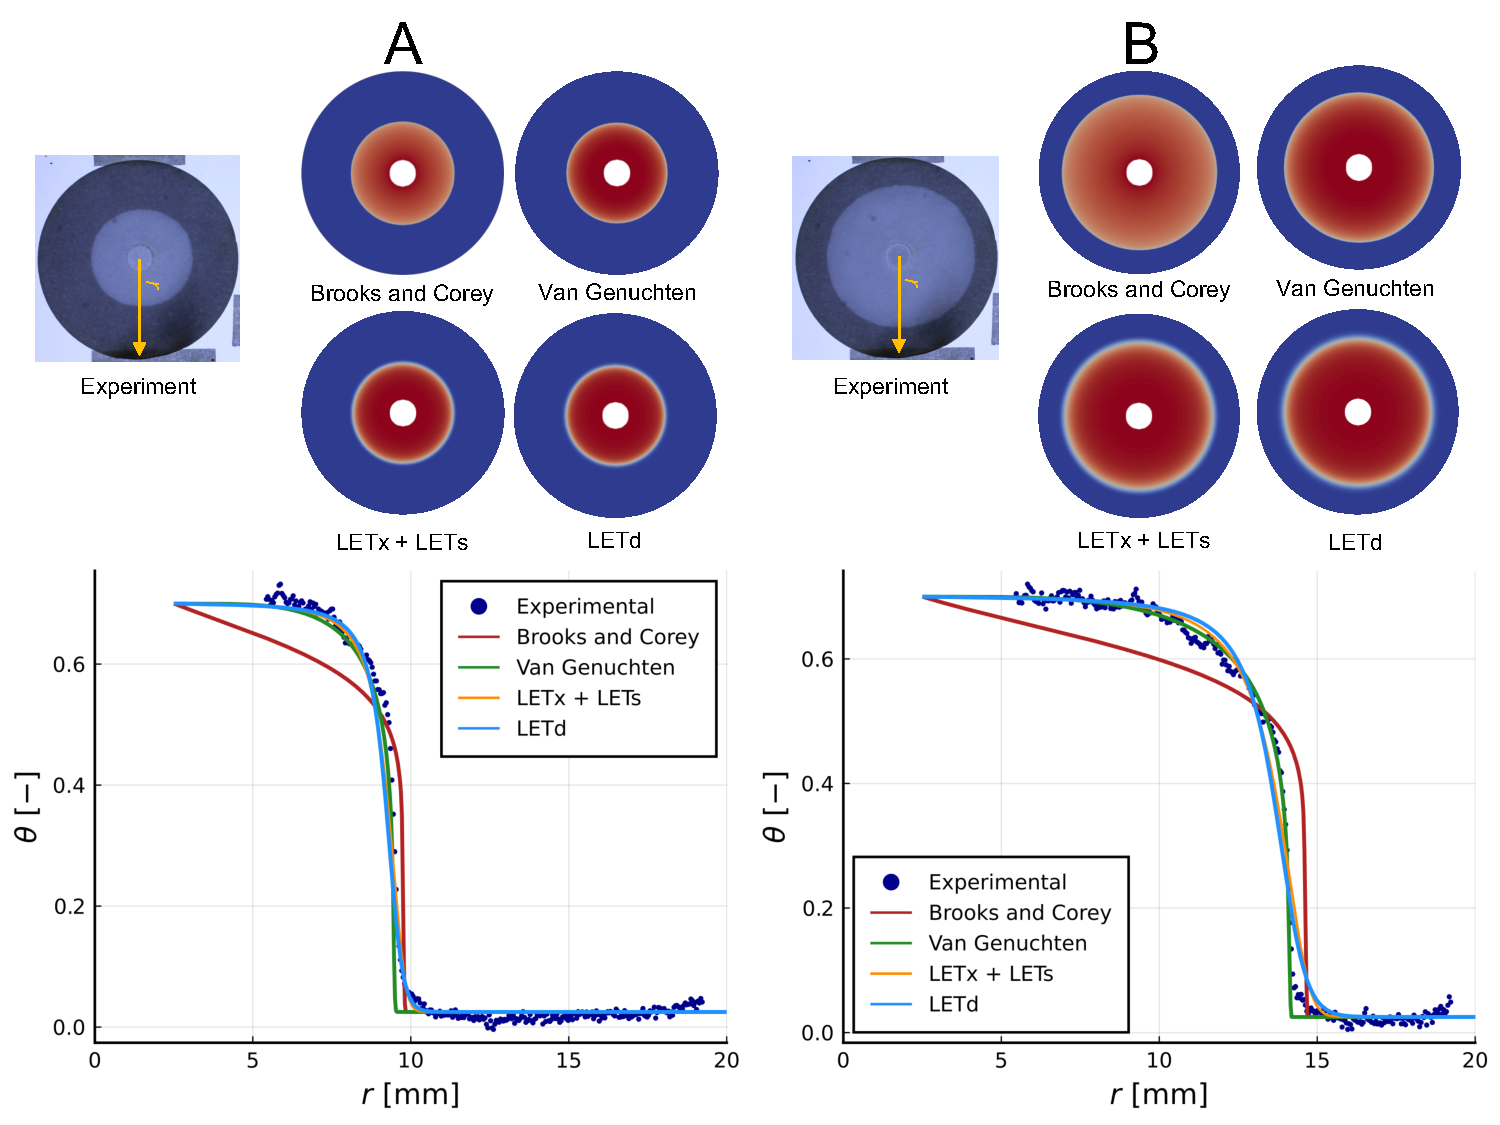
\includegraphics[width=.85\textwidth]{pics/shape_figures4.pdf}
    \caption{Ensayos experimentales y numéricos con diferentes modelos capilares de flujo de imbibición en papel Whatman \# 1.}
    \label{fig:validity}
\end{figure}    

\subsection{Flujo reactivo en medios microestructurados}
Dada la experiencia del grupo en dos tecnologías particulares, como son los análisis de flujo lateral~\cite{schaumburg2018numerical} y la electroforesis capilar tanto en canales abiertos~\cite{damian2018open} como en papel y medios porosos~\cite{schaumburg2020comprehensive}, existe una gran conocimiento acerca de la implementación de diferentes tipos de reacciones como términos fuente en la ecuación de transporte, y el acople de ésta con la solución de flujo transientes y estacionarios. Recientemente, el grupo ha colaborado con la extensión del código \texttt{porousMultiphaseFOAM}~\cite{porousMultiphaseFoam} para la inclusión de una ecuación de transporte multiespecie en el régimen de flujo no saturado resuelto mediante dicha herramienta. Esta ecuación de transporte multiespecie incluye además términos reactivos de orden variable que permiten modelar diversos tipos de reacciones. Por ejemplo cinéticas discontinuas tipo Liesegang en medios porosos~\cite{PFCHGG}. %Paralelamente, se han realizado pruebas de verificación de compatibilidad para la interacción entre la biblioteca reaktoro~\cite{reaktoroweb} y \of{}.


\subsection{Generación de microgotas}
Se elaboró un compendio de aproximaciones empíricas y semi--empíricas presentes en la literatura para obtener un calculador de generadores para su diseño, basado en las diferentes propuestas. Dicho calculador tiene una interfase web, cuya maqueta se encuentra terminada, a la espera de la carga de las ecuaciones compendiadas y servirá de punto de partida para la verificación del resto de las herramientas a desarrollar. Se implementaron  prototipos numéricos básicos de generadores de gotas en  flujo bifásico mediante la herramienta Basilisk~\cite{popinet2015quadtree}, quedando demostrada su utilidad para la aplicación objetivo\cite{Marengo2019generation}.
\begin{figure}
    \centering
    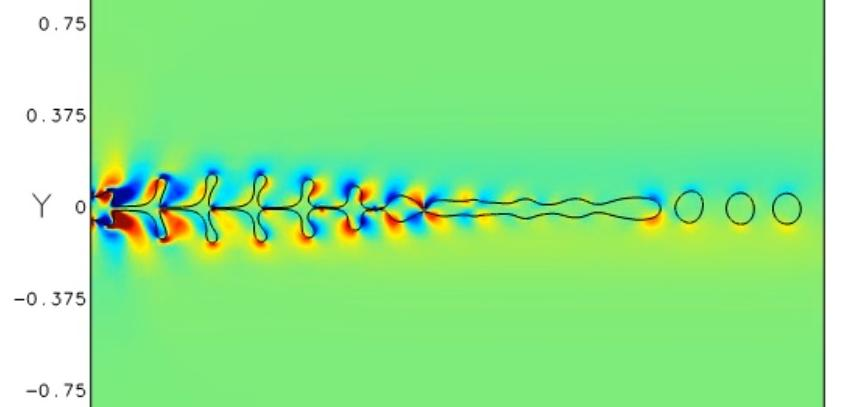
\includegraphics[width=.65\textwidth]{pics/microgotas.jpeg}
    \caption{Experimentos numéricos de generación de gotas bifásicas en sistemas aceite-agua utilizando \texttt{Basilisk}}
    \label{fig:basilisk}
\end{figure}   

\newpage

\section{CONSTRUCCION DE LA HIPOTESIS y JUSTIFICACION GENERAL DE LA
METODOLOGIA DE TRABAJO} 

{\it (máx 1 pág.)
A partir de lo expuesto en la introducción y los datos preliminares proponer la hipótesis de trabajo y justificar la metodología propuesta.}


Los problemas a resolver pueden ser descriptos mediante ecuaciones diferenciales en derivadas parciales con respecto al tiempo y a las coordenadas espaciales. En el caso del flujo de fluidos, se considerarán las ecuaciones de NS para el caso incompresible, viscoso, newtoniano e isotérmico, con las condiciones de borde propias de cada caso. 
%% Para el caso del flujo capilar de llenado en medios porosos se utiliza una simplificación de las ecuaciones de NS en un esquema tipo Darcy con permeabilidades y porosidades distribuidas.
%% Uno de los principales inconvenientes de esta formulación diferencial es la dificultad para
%% representar adecuadamente las variaciones del campo de velocidad ante discontinuidades en la porosidad de los materiales, por lo que se propone enriquecer esta formulación con términos adicionales de tipo Brinkmann o Forchheimer~\cite{Mendez09}.
%% En el caso de las ecuaciones de transporte, se utiliza un modelo de conservación tipo advectivo-difusivo-dispersivo-reactivo donde los esquemas reactivos varían de acuerdo a la aplicación (ácido-base, antígeno-anticuerpo, hibridación, entre otros).

%% %
Las metodologías de discretización numérica a aplicar para resolver las ecuaciones antes mencionadas serán las de los métodos de volúmenes finitos y elementos de borde, aptos para abordar la resolución de problemas sobre dominios de geometrías de forma general. Otras metodologías de simulación serán utilizadas para la resolución de problemas auxiliares o para la verificación de resultados.
%% %

Las diferentes técnicas a aplicar para simular flujos con interfases móviles involucran la resolución de dos o más problemas acoplados. En el caso general, se empleará una metodología de acoplamiento débil, que consiste en resolver numéricamente cada campo por separado en cada paso de tiempo, mediante programas específicos que coordinan el intercambio de información entre ellos.


%% En el caso particular de BEM, una t\'ecnica num\'erica que recurre al uso de las funciones de Green, resulta ventajoso en su aplicación a problemas lineales, en particular los extendidos a infinito, que dan lugar a ecuaciones integrales de borde, que suelen reducirse a integrales en el borde (o contorno o frontera) del dominio. Para la determinación de acciones del fluido (tracciones) sobre los cuerpos involucrados no requiere otras instancias de solución, siendo apto para geometr\'{\i}as intrincadas, especialmente en 3D.

Los programas se desarrollarán en lenguajes o códigos que permiten la programación orientada a objetos, tal que los módulos o librerías que resuelven diferentes problemas físicos pueden comunicarse mediante aplicaciones diseñadas específicamente, y considerando su ejecución en estructuras de cálculo distribuido como los clusters presentes en CIMEC. Este esquema modular permite, por ejemplo, el intercalado de instancias de movimiento de malla sin afectación significativa de la estructura del programa. 

Los resultados obtenidos mediante las técnicas antes mencionadas serán comparados con resultados experimentales o analíticos disponibles en la literatura, o accesibles mediante intercambios con otras instituciones asociadas al grupo colaborador. Se realizarán también comparaciones con otros resultados numéricos. 
De los resultados de la comparación se establecerá el grado de precisión con el cual pueden representarse los problemas que pueden resolverse con las metodologías estudiadas.

\newpage

\section{TIPO DE DISEÑO DE INVESTIGACION Y MÉTODOS}
\iftrue
{\it (máx. 9 pág.)
Se deberá organizar el estudio propuesto en secciones mayores, correspondientes a los objetivos específicos, y, secciones menores, correspondientes a experimentos específicos para explicar:
1. La base racional de cada experimento o estudio propuesto.
2. Como se llevara a cabo el experimento o estudio.
3. Que controles se usarán – en caso de ser necesarios - y porqué.
4. Que técnicas específicas se utilizarán discutiendo aspectos más críticos o
modificaciones de manipulaciones habituales: Respecto a las técnicas y
tecnologías empleadas (los métodos) si son parte del patrimonio del grupo y
han sido descriptas en publicaciones propias o en los datos preliminares - no
deberán detallarse y solo deberá citarse la fuente-. Explicar si se recibirá
apoyo técnico de colaboradores.
5. Como se interpretaran los datos a la luz de lo que se quiere estudiar y como
se contrastará con la hipótesis de trabajo.
6. Tratar de evaluar los potenciales problemas y limitaciones de la metodología y
técnicas propuestas y en lo posible proponer alternativas.}


\textcolor{magenta}{Tomado de PIP2020}
\fi




\subsection{Descripción de las metodologías y estrategias particulares}

Como se estableció en la sección anterior, los problemas a resolver son descriptos mediante ecuaciones diferenciales en derivadas parciales con respecto al tiempo y el espacio en el marco de la mecánica del continuo. Básicamente, se trata de un conjunto de ecuaciones diferenciales acopladas quedando el problema completamente definido cuando se fija el dominio de aplicación, las condiciones iniciales y de borde. En el caso del flujo de fluidos, se considerarán las ecuaciones de Navier--Stokes para el caso incompresible, viscoso, newtoniano e isotérmico. 

La formulación e implementación de los cálculos se hará utilizando el Método de Volúmenes Finitos (MVF) en las plataformas \of{} y Code\_Saturne. El MVF consiste en la discretización de la ecuaciones de conservación en forma débil, es decir mediante el balance de flujos en las caras de un dominio dividido en una cantidad finita de volúmenes, lo cual da lugar a su nombre. El método es inherentemente conservativo, cualidad de suma importancia cuando se desean resolver problemas de flujo incompresible y/o transporte de especies que reaccionan. 
Una vez definidos los dominios, las ecuaciones, las propiedades reológicas y fisicoquímicas, y las condiciones iniciales y de borde en las plataformas mencionadas, se resolverán en computadoras personales, clusters locales~\cite{C3} o supercomputadoras asociadas al SNCAD~\cite{rf:sncad}, según la magnitud del problema.

Se detallan a continuación algunas particularidades de los modelos matemáticos y estrategias computacionales a utilizar asociadas a cada objetivo particular, constituyendo cada uno un paquete de tareas, con su consecuente correlato en el cronograma propuesto en la siguiente sección.

\subsubsection{Superficie libre}
\label{sec:suplibre}

La estrategia prevista para la solución de flujos con superficie libre es la de un {\it volume of fluid} (VOF) resuelto mediante volúmenes finitos. 

Se propone generar una metodología para el cálculo de solicitaciones, tanto distribuidas como integradas, en contornos u objetos inmersos en flujos con interfases móviles~\cite{Kamath2021sloshing}, que involucren los efectos de la presión $p$ y de las tensiones tangenciales $\tau$. Por ejemplo, para el caso integrado en una superficie $\Omega$, 
\begin{equation}
\mathbf{F} = \int_\Omega (-\mathbf{n}p+\mathbf{n}\cdot \tau)\ \mathrm{d} \Omega,
\end{equation}
%
en la cual $\mathbf{n}$ es el versor unitario hacia el fluido de $\Omega$. 
La obtención de estas cantidades permitirá a su vez la estimación de los efectos de fuerzas y momentos en instalaciones de almacenamiento~\cite{Kang2019}  o sistemas de transporte. %% cambiar refs. por nuevas

Tanto la dinámica de las interfases móviles como las solicitaciones en superficies sólidas se ven afectadas por los efectos de la turbulencia que se produce en los flujos de interés. Actualmente, se dispone de distintas aproximaciones para tener en cuenta tales efectos, típicamente {\it Reynolds-Averaged Navier-Stokes} (RANS) y {\it Large Eddy Simulation} (LES), tanto en Code$\_$Saturne como en \of{}. La pertinencia de los modelos y parámetros a definir requiere estudios de convergencia y la validación con resultados experimentales, que se llevarán adelante en virtud de intercambios con la Dra. Marcela Cruchaga y otros investigadores de la USACH, quienes habitualmente realizan ensayos en laboratorio para problemas de agitación e interacción fluido-estructura. 
%% Editado hasta acá por Laura

Por otro lado, ...

El estudio computacional de dominios con fronteras abiertas, tal como cierta sección de un canal a superficie libre, se ve afectado por efectos numéricos no deseados originados en los contornos artificiales impuestos debido a la reflexión de olas que en ellos se produce. Por este motivo, es de interés el desarrollo de un estanque de olas numérico (NWT, por sus siglas en inglés)~\cite{Hu20179}, caracterizado por (i) generadores de ondas de ingreso y (ii) condiciones de borde  absorbentes, que evitan reflexiones espurias en los contornos ficticios. % ver con Gustavo
%
En este sentido, se estudiarán modelos de producción de ondas con el propósito de reproducir el oleaje que se registra en condiciones naturales~\cite{Li2019,Romanowski2019,Stagonas2018}. A tal fin, las técnicas a emplear deberán considerar una regla de desplazamiento de ingreso para la superficie libre, y una regla para definir las velocidades en el mismo contorno. 
En lo referido a reflexiones espurias de olas en contornos artificiales, producidas tanto en secciones de ingreso como de salida en régimen subcrítico, es preciso dotar al NWT de regiones diseñadas para evitar tales reflejos. Estas regiones pueden contar con propiedades absorbentes en general~\cite{Paz201152}, o definirse con condiciones de contorno variables~\cite{rf:storti-dynbc}. Técnicas similares~\cite{Chen2014numerical,Deng2019} serán tomadas como referencia para la validación y/o contraste. 
Empleando estas técnicas, la caracterización de empujes hidrodinámicos sobre objetos sumergidos total o parcialmente, permitirán calcular acciones dinámicas en los objetos sumergidos~\cite{Suja2018} sin afectarlas con reflexiones espurias. 

%% ------------ grios ----------- %%
%% Párrafo sobre rotura de olas
También resulta fundamental contar con modelos numéricos que permitan resolver aquellos casos en los cuales las olas rompen sobre estructuras parcialmente sumergidas, comoocurre sobre los pilares de estructuras offshore. En el análisis dinámico de dichas estructuras resulta fundamental considerar el desarrollo temporal de la fuerza (su historia) además de su intensidad. Debido al breve lapso de tiempo en el que se desarrolla el fenómeno de rotura, el análisis detallado resulta complejo, si bien se han desarrollado diversos modelos analíticos~\cite{wienke_breaking_2005}, estudios experimentales~\cite{irschik_belastung_2012,tai_experimental_2019} y también análisis numéricos~\cite{qu_evaluation_2021}.
%%
Desde el punto de vista numérico resulta fundamental considerar condiciones de borde específicas que permitan generar grupos o trenes de ondas enfocados (i.e. focused wave groups) ya que modificar la ubicación del foco con respecto de la estructura considerada permite analizar distintos tipos de impactos de la ola~\cite{hu_numerical_2016,hu_investigations_2017}. Por otro lado, el estudio de olas extremas y su correcta representación analítica y numérica también resultan fundamental en el proceso de dise\~no de estructuras offshore. En este sentido, se empleará la teoría NewWave~\cite{tromans_new_1991} la cual permite simular de forma determinística olas extremas~\cite{vyzikas_numerical_2018} tanto en aguas profundas como intermedias o de poca profundidad~\cite{whittaker_average_2016}.
%%
%%En los casos de olas que no rompen la ecuación de Morison resulta apropiada en la medida que las esctructuras presenten una determinada esbeltez en relación a la longitud de las olas. Sin embargo, en los casos de olas rompientes dicha ecuación no es suficiente ya que no considera la componente dinámica de la carga ({\it slamming} sino sólo la parte cuasi-estática~\cite{wienke_breaking_2005}.
%%
%% ------------ end grios ----------- %%


Los métodos estudiados en esta sección Como parte de la metodología, se prevé establecer una comparación con las estrategias a proponer en la Sec.~\ref{sc:fsi} en cuanto a precisión y escalabilidad en entornos de HPC a fin de contar con elementos de decisión al momento de optar por una u otra herramienta de cálculo. 

\subsubsection{Interacción fluido estructura con cuerpos inmersos}
\label{sc:fsi}

La interacción fluido-estructura, en este caso asumiendo cuerpos rígidos inmersos en un fluido incompresible y newtoniano, ha sido abordada en el grupo de trabajo mediante un término de permeabilidad, o de Darcy, en las ecuaciones de NS:
%
\begin{align}
\rho(\frac{\partial {\bf u}}{\partial t} + {\bf u} \cdot \nabla {\bf u}) &= - \nabla p + \mu \ \Delta {\bf u} + \kappa \left( {\bf u} - {\bf u_{\rm b}}\right)\label{eq:NS-LD}  \\ 
\nabla \cdot {\bf u} &= 0
\end{align}
%
siendo $\rho$ y $\mu$ la densidad y la viscosidad dinámica del fluido, respectivamente, ${\bf u}$ la velocidad del fluido, $p$ la presión y ${\bf u}_{\rm b}$ la velocidad del sólido inmerso. En el término de Darcy, $\kappa$ es una resistividad hidraúlica ficticia, que en las celdas ocupadas por el cuerpo es $\kappa>0$, mientras que en el fluido es $\kappa = 0$~\cite{ZamoraENIEF19,Zamora2021}. 

La resolución de la Ec.~(\ref{eq:NS-LD}) se lleva a cabo discretizando en volúmenes finitos mediante Code$\_$Saturne~\cite{Saturne2020}, para lo cual se ha implementado el término adicional a NS en una rutina de usuario. Esta representación facilita además el cálculo de las fuerzas del fluido sobre los cuerpos inmersos, mediante la integral del término $\kappa \left( {\bf u} - {\bf u_{\rm b}}\right)$, que es no nulo únicamente en la región ocupada por el sólido, gracias a la aplicación de una máscara binaria. En el caso de cuerpos móviles, los efectos inerciales son tenidos en cuenta en la suma global de fuerzas. A partir del desarrollo actual, en el cual los desplazamientos de los cuerpos pueden ser nulos o impuestos por una regla externa, se propone la solución de la interacción sólido-fluido para cuerpos libres, para lo cual se requiere resolver la dinámica del sólido mediante una rutina o código externo para resolver la ecuación de Newton-Euler.  

%
Las alternativas a considerar para resolver el movimiento del sólido incluyen el acoplamiento con librerías externas de desarrollo externo, como ser: i) el código 3DLSDEM~\cite{KAWAMOTO2016,jerves2016effects}; ii) un solver tipo Newton, desarrollado en la USACH~\cite{Ortega2017} para cuerpos esféricos; iii) rutinas propias. Cada una de las alternativas será evaluada a fin de establecer la posibilidad de integración con la metodología en su estado actual, convergencia, escalabilidad y estrategias de identificación de la posición del cuerpo o los cuerpos representados. Debe destacarse que valores excesivos de la penalización $\kappa$ pueden producir inestabilidades numéricas en el cálculo de las fuerzas, y que la solución de la dinámica de cuerpos rígidos que impactan entre sí y con contornos condiciona severamente el tamaño del paso de tiempo. 

 La validación se realizará a distintos niveles de complejidad, por ejemplo con códigos de contornos explícitamente definidos en el mismo entorno de Code$\_$Saturne~\cite{Saturne2020}, o mediante la solución de benchmarks tales como los de sedimentación de partículas esféricas, o  comparando con resultados experimentales disponibles mediante intercambios con la USACH y otros organismos o institutos de investigación. 
%

En los casos en los que el sólido atraviesa una interfase entre dos fluidos, a la metodología antes mencionada se adiciona la dinámica particular de la superficie libre representada mediante VOF. Esta representación, que incluye tanto la fase líquida como la fase gaseosa, no requiere tratamiento particular en el caso del cuerpo. No obstante, para una representación apropiada de la superficie libre, será preciso estudiar el nivel de refinamiento necesario en torno a los cuerpos flotantes~\cite{TanLoh2018}. \textcolor{red}{completar este párrafo}

La aplicación de esta metodología, al finalizar las etapas antes mencionadas, se encuentra prevista sobre prototipos de generadores de energía undimotriz, 



\subsubsection{Flujo en medios porosos}
En el estudio del flujo en medios porosos, para las aplicaciones a las que se enfoca este proyecto, conviene a priori separar entre regímenes de flujo saturado e insaturado.

Para el caso de flujo en medios porosos saturados, se utiliza la siguiente generalización de la ecuación de Navier--Stokes para la conservación de momento:
\begin{align}
\label{eq:NS_PM1}
\frac{\tau^2}{\phi}\frac{\partial \mathbf{u}}{\partial t} + \frac{\tau^2}{\phi}\mathbf{u}\cdot\nabla\left(\frac{\mathbf{u}}{\phi} \right) = \frac{\mu}{\rho}\nabla^2\left(\frac{\mathbf{u}}{\phi}\right)-\frac{1}{\rho}\nabla p +\frac{\mu\tau}{\rho}\frac{\mathbf u}{K}
\end{align}
donde $\tau$ y $\phi$ representan la tortuosidad y la porosidad del medio, $K$ es la permeabilidad de Darcy, $\rho$ es la densidad del fluido, y $\mathbf{u}$ y $p$ los campos incógnita de velocidad y presión. Cabe destacar que esta ecuación es la más general que se conoce para este tipo de problemas y simplemente despreciando los términos correspondientes a cada caso (\textbf{no todos los términos son no-nulos simultáneamente}), se llega a formulaciones conocidas y muy utilizadas como la formulación de Darcy, Darcy--Forchheimer, o Darcy--Brinkman. Esta implementación se encuentra funcional y verificada en el código desarrollado y mantenido por el grupo \texttt{electroMicroTransport}~\cite{damian2018open,GERLERO2021108143,gerlero2021numerical}.

Una alternativa a estas formulaciones de propiedades del medio poroso promediadas en el espacio son los modelos multiescala basados en homogeneización ya sea a través de la ecuación de Navier--Stokes~\cite{blanco2017homogenization} o a través de una reformulación de las relaciones de clausura entre la saturación, permeabilidad y presión capilar en la ecuación de Richards. Este último enfoque es novedoso y uno de los ejes principales de una tesis de una becaria doctoral del grupo.

En el caso de flujo en régimen insaturado, tanto el problema diferencial como el numérico crecen en complejidad. En estos casos conviene utilizar la formulación conocida como ecuación de Richards~\cite{Richards}, cuya expresión simplificada para medios homogéneos es:
\begin{equation} \label{eq:Richards}
    \frac{\partial\theta}{\partial t}-\frac{K \rho g}{\mu}\nabla\cdot\left(\frac{K_r}{C}\nabla\theta\right) = 0
\end{equation}
donde $\theta$ es la saturación del medio y, $k_r$ y $C$ representan la permeabilidad relativa y la \textit{capacidad capilar del medio}. Estos dos últimos parámetros son función de la saturación $\theta$, y dicha dependencia es objeto de estudio, siendo los modelos más utilizados los de Brooks--Corey~\cite{BrooksAndCorey}, Van Genuchten~\cite{VanGenuchten} y LET~\cite{lomeland2018overview}. Para el caso de dominios 1D, el grupo ha desarrollado y validado el software \texttt{fronts}\cite{frontsweb,fronts} que permite resolver de manera extremadamente eficiente tanto los problemas directos, como estimaciones de las funciones $k_r(\theta)$ y $C(\theta)$ a partir de datos experimentales\cite{gerlero2022validity}. Para casos 2D y 3D, el grupo cuenta con experiencia en el desarrollo y la utilización de la herramientas  \texttt{porousMultiphaseFOAM}~\cite{porousMultiphaseFoam} que permite la resolución de la ecuación de Richards y su acoplamiento con el transporte de escalares. 

Cabe destacar que el grupo viene desarrollando y validando técnicas numéricas para flujo en medios porosos desde 2015 tomando como material de estudio el papel para aplicaciones microfluidicas. El estudio de hormigones drenantes comprende el desarrollo de tareas que permitan el acondicionamiento de las mencionadas técnicas (tanto experimentales como numéricas) a las particularidades de este material. Sin embargo las técnicas se han desarrollado desde un principio sin perder de vista su generalidad y aplicabilidad en otros materiales y campos, lo que permite vislumbrar una gran factibilidad en el corto plazo. Para la caracterización hidráulica de los materiales y validación de modelos de flujo, se cuenta con la colaboración permanente del Dr. Raúl Urteaga del IFIS-Litoral (UNL--CONICET)\cite{gerlero2022validity,franckprecise}


\subsubsection{Flujo reactivo}

El flujo reactivo en medios porosos se modela mediante el principio de conservación de masa. Dicha conservación, plantea que la variación temporal de la masa de un determinado componente $C^j$, es equivalente a la superposición de los diferentes tipos de flujo intervinientes, más un término reactivo que propicia la generación o extinción de dicho escalar. Formalmente, la concentración $C^j$, se obtiene resolviendo la siguiente ecuación:
\begin{align}
\label{eq:TranpPorous}
\frac{d(C^j\phi)}{dt}&=-\mathbf \nabla \cdot\left(\frac{\mathbf{u}}{\phi} (C^j\phi)-\left(\frac{D^j_0}{\tau^2}+s_f|\frac{\mathbf{u}}{\phi}| \right) \nabla \left(C^j \phi\right)\right)+r^j\phi
\end{align}
donde $s_f$ es el coeficiente de dispersión y $r^j$ el término reactivo.
Para este caso, los diferentes tipos de flujo considerados son (en orden de aparición en la ecuación desde la izquierda) el flujo advectivo, el flujo difusivo, y el flujo dispersivo. Esta ecuación ya se encuentra implementada y validada en el código  \texttt{electroMicroTransport}. Los términos reactivos pueden ser de las naturalezas más variadas, como adsortivos, ácido--base, de hibridación, enzimáticos, inmunológicos, etc~\cite{schaumburg2020comprehensive}. 

En este caso, los mecanismos de reacción a estudiar revisten una complejidad moderada, dada la actividad de alta especificidad propia de las superficies catalíticas~\cite{regenhardt2020monolithic}. La complejidad que requieren las nuevas implementaciones a los fines de contemplar la acción catalítica de la superficie requiere cuantificar la interacción de diversos procesos como la adsorción de los reactivos, el tiempo de adsoción/reacción, la liberación del sitio de catálisis, entre otros. La colaboración con el Dr. Camilo Meyer de INCAPE (UNL--CONICET) permitirá validar experimentalmente los modelos en reactores microestructurados monolíticos.

Es destacable que el grupo de trabajo tiene vasta experiencia en el desarrollo de algoritmos para la resolución tanto del flujo de fluidos como de diversos mecanismos de transporte no-tradicionales como dispersión mecánica, electromigración, dispersión electroforética, patrones de Liesegang entre otros~\cite{damian2018open,schaumburg2020comprehensive}.  


 
\subsubsection{Simulación de generadores de microgotas}

Para estudiar la dinámica en la formación de microgotas, tanto la fase continua como la dispersa, se modelan como incompresibles, con propiedades reológicas constantes e inmiscibilidad perfecta. El número capilar indica en que medida los efectos de tensión superficial serán o no dominantes para la formación de gotas monodispersas, se calcula como
\begin{align}
    Ca=\frac{\mu|\textbf{u}|}{\gamma}
\end{align}
donde $\gamma$ es el coeficiente de tensión superficial. Dicho número capilar representa el núcleo de todos los modelos semi-empíricos presentes en la literatura, que se compendian en el calculador web que se encuentra en desarrollo.

Cuando se utilizan modelos teóricos basados en ecuaciones de conservación y modelos constitutivos verificados, el primer paso es la cuantificación de los efectos de la tensión superficial. Estos efectos se consideran a partir de la inclusión de un término de fuerza superficial $\mathbf{F_s}$ a la ecuación de Navier--Stokes para la conservación de momento. Esta fuerza se calcula como:
\begin{align}
    \mathbf{F_s}=\int_{S(t)}\gamma\kappa(x,t)\mathbf{n}dS
\end{align}
donde $\kappa(x,t)$ la curvatura de la interfase $S(t)$, cuyo vector normal es $\mathbf{n}$. La curvatura se calcula como:
\begin{align}
\kappa(x,t)=-\mathbf{\nabla\cdot n}
\end{align}
y el vector normal como:
\begin{align}
\mathbf{n}=\frac{\nabla \alpha}{|\nabla \alpha|}
\end{align}
donde $\alpha$ es la fracción másica de alguna de las dos fases definida de la manera estándar en el método de VOF.
El desafío numérico de este esquema está en calcular de manera correcta las curvaturas para poder calcular de manera adecuada la fuerza actuante y determinar así el valor de $\alpha$ en todo en dominio en cada instante de tiempo. 

Para los prototipos numéricos basados en esta estrategia, la primera alternativa para el manejo de la interfase es VOF. Aquí se utilizará una herramienta de simulación numérica de alto desempeño basada en MVF llamada \texttt{Basilisk}~\cite{popinet2015quadtree}. \texttt{Basilisk} es una herramienta de código abierto, paralela, programada en $C$, orientada a flujo multifásico, basado en el método de VOF y con diferentes estrategias para el tratamiento de las interfases, como el refinamiento adaptativo basado en \textit{octrees} y algoritmos de alto orden para el cálculo de curvaturas. 

Ya se cuenta con resultado propios que demuestran la correcta capacidad \texttt{Basilisk} para modelar los sistemas de generación de microgotas monodispersas en los regímenes de $Ca$ y $Re$ típicos de las aplicaciones microfluídicas a considerar. Se propone continuar con el uso de \texttt{Basilisk} para simular diversas condiciones de operación, topologías y regímenes de flujo tanto para sistemas O/W como W/O. El costo computacional de estas simulaciones basadas en VOF, es por ahora incompatible con procesos de diseño y prototipado rápido. Siendo necesario elaborar estrategias con menor costo~\cite{iqbal2020effect}. 

En el caso de los generadores de microgotas, excepto por los generadores coaxiales, resulta inadecuada la reducción dimensional~\cite{shao2013controlled}. Por otra parte, y sobre todo en el método de VOF, reducir la calidad de la malla puede resultar en la divergencia casi inmediata de las soluciones~\cite{mora2019numerical}.

Otra estrategia para disminuir el costo computacional, es tener aproximaciones menos complejas a la física de los problemas. En este marco se encuentra el método de dos fluidos. Este método, de menor costo computacional que VOF, basa su estrategia en incorporar leyes de cierre (generalmente pseudo-empíricas) para ajustar los esfuerzos en la interfase de los fluidos, sin necesidad de resolver la zona con tanta precisión. Es sabido que el método de dos fluidos presenta muchos problemas de estabilidad y es muy sensible a la forma matemática de las leyes de cierre propuestas~\cite{de2017two}. Se investigará si se puede configurar una red neuronal para funcionar con mayor potencialidad que una simple regresión lineal a partir de los datos de VOF (mediante \texttt{Basilisk}) para enriquecer los modelos de dos fluidos. Para ello deben desarrollarse estrategias adecuadas que permitan la incorporación de parámetros reológicos y principios de conservación~\cite{hadikhani2020numerical}. 

Se investigará acerca de las particularidades informáticas de esta implementación, a los fines de lograr arquitecturas de la red y estructuras de datos acordes a los requerimientos. Se dispone de facilidades experimentales para validar los modelos a través de la permanente cooperación con el Dr. Federico Schaumburg del laboratorio de prototipado microfluídico de INTEC (UNL--CONICET).

\subsection{Acerca del grupo de trabajo}

\textcolor{red}{revisar: Marcela Cruchaga. }

\textcolor{red}{revisar: Gente relacionada con fonarsec/UTN-FRBB. }

Como se ha indicado en secciones previas, el grupo responsable de la propuesta se compone de investigadores formados (adjuntos, independiente y principal en CIC CONICET) con lugar de trabajo en CIMEC.
%
En particular, J D'El\'{\i}a es Responsable T\'{e}cnico ante el SNCAD de los clusters de c\'{o}mputo en la UE. 
%
En el grupo colaborador se incluyen a aquellos investigadores formados que colaboran ya sea en tareas experimentales de validación informadas y proyectadas: Federico Schaumburg (INTEC), Raúl Urteaga (IFIS), y Hugo G. Castro (IMIT, Chaco), como en la formulación matemática y numérica en BEM: el Inv. Adjunto Ezequiel López y la Inv. Asistente Sofía Sarraf (dirigida por J. D'Elía), ambos en el IITCI (UNCo-CONICET), Universidad Nacional del Comahue (UNCo), Neuquén.
%
Completan el grupo colaborador becarios doctorales dirigidos por los integrantes del grupo responsable que se encuentran trabajando temáticas afines al proyecto. 
%
Otros investigadores con los cuales hay vínculos de colaboración establecidos son Marcela Cruchaga (USACH) y Marco Schauer (Institut für Statik, TU Braunschweig, Alemania)
\cite{Battaglia2018,Cruchaga2013}. Poner trabajos en congresos 2021 en común. 
%
\textcolor{red}{Vinculaciones por BIOTRAFO?}



\newpage

\section{CRONOGRAMA DE TRABAJO}
\iftrue
{\it (máx. 1 pág.)
Se presentará una tabla de doble entrada con las tareas desagregadas y los tiempos estimados que consumirán.}
\fi
% Para facilitar la lectura de la representación gráfica del 
% cronograma se presenta antes un listado de tareas que guardan 
% relación con las presentadas en la sección anterior.

\def\b{\rule{0.3cm}{0.1cm}}
%\def\pb#1{\parbox{7.0truecm}{#1}}

\def\c{\rule{0.3cm}{0.05cm}}
\renewcommand\baselinestretch{0.25}  % interline

{\small \subsection{Listado de tareas (para facilitar la lectura de la presentación gráfica)}
Se listan los miembros del GR a cargo de cada paquete de tareas
\begin{itemize}[noitemsep]
%% %
%% % \paragraph*{Tarea 1. Flujo con superficie libre}
\item Tarea 1. Flujo con superficie libre: 
   \begin{itemize}[noitemsep]
   \item Tarea 1.1. Captura de interfase para volúmenes finitos en computación de alto desempeño
   \item Tarea 1.2. Regularización de la función marcadora para captura de interfase 
   \item Tarea 1.3. Determinación de acciones sobre contornos y cuerpos sumergidos
   \item Tarea 1.4. 
   \item Tarea 1.5. 
   \item Tarea 1.6. 
  \end{itemize}
    %\end{itemize}
%%   %
%% % \paragraph*{Tarea 2. Fenómenos de transporte en medios porosos}
\item Tarea 2. Interacción Fluido estructura. 
   \begin{itemize}[noitemsep]
   \item Tarea 2.1. 
   \item Tarea 2.2. 
   \item Tarea 2.3. 
   \end{itemize}
%%   %
%% % \paragraph*{Tarea 3. Flujos con objetos inmersos mediante BEM}
\item Tarea 3. Flujo en medios porosos:
   \begin{itemize}[noitemsep]
   \item Tarea 3.1. Caracterización experimental de diferentes hormigones drenantes. 
 \item Tarea 3.2. Implementación de modelos en flujo saturado.
   \item Tarea 3.3. Implementación de modelos en flujo saturado.
   \item Tarea 3.4. Prototipado numérico de elementos constructivos de interés ingenieril.
      \end{itemize}
%%   %
%% % \paragraph*{Tarea 5. Flujo con objetos inmersos e interacción fluido-estructura}
 \item Tarea 4. Flujo reactivo: 
   \begin{itemize}[noitemsep]
   \item Tarea 4.1. Implementación de modelos catalíticos heterogéneos.
   \item Tarea 4.2. Verificación de consistencia y estabilidad numérica de la implementación de la ecuación de transporte.
   \item Tarea 4.3. Desarrollo de modelos de flujo multiescala.
   \item Tarea 4.4. Validación con reactores monolíticos.
   \item Tarea 4.5 Resolución de prototipos acoplados flujo en hormigones drenantes--reacciones de descontaminación.
   \end{itemize}
%%   %
 \item Tarea 5. Simulación de microgotas: 
   \begin{itemize}[noitemsep]
   \item Tarea 5.1. Compendiado de modelos empíricos y semi-empíricos.
   \item Tarea 5.2. Implementación de modelos en calculador web.
   \item Tarea 5.3. Implementación de modelos VOF en Basilisk.
   \item Tarea 5.4. Estudio de factibilidad y sensibilidad de modelos de dos fluidos.
   \item Tarea 5.5. Acoplamiento VOF-2F-ML. 
   \end{itemize}
 \end{itemize}}

\subsection{Presentación gráfica del cronograma}
\begin{center}

{\centering
\begin{tabular}{|p{1cm}|c|c|c|c|c|c|c|c|}
  \cline{2-9}
  \multicolumn{1}{c}{} & \multicolumn{8}{|c|}{Meses}\\
  \hline
  Tarea & 1-3 & 4-6 & 7-9 & 10-12 & 13-15 & 16-18 & 19-21 & 22-24 \\
  \hline
  \hline
  { 3.1}  & \b  & \b & \b &  &  &   & &  \\
  \hline
  { 3.2}  &  & \b & \b & \b &  &   & &  \\
  \hline
  { 3.3}  &  &  &  &  &  & \b  &\b &\b  \\
  \hline
  { 4.1}  &  &  &\b&\b&\b&   & &  \\
  \hline
  { 4.2}  &  &  &  &  &  &\b&\b&\b  \\
  \hline
  { 4.3}  &  &  &  &  &  & \b  &\b &\b  \\
  \hline
  { 5.1}  & \b &\b  &  &  &  &   & &  \\
  \hline
  { 5.2}  &  &  & \b & \b &\b  &   & &  \\
  \hline
  { 5.3}  &  &  &  &  &  & \b  & \b&\b  \\
  \hline
\end{tabular}}

{\centering
\begin{tabular}{|p{1cm}|c|c|c|c|c|c|c|c|}
  \cline{2-9}
  \multicolumn{1}{c}{} & \multicolumn{8}{|c|}{Meses}\\
  \hline
  Tarea & 25-27 & 28-30 & 31-33 & 34-36 &37-39& 40-42 & 43-45 & 46-48 \\
  \hline
    { 3.3}  & \b &  &  &  &\b  & \b  & &  \\
  \hline
  { 3.4}  &  &\b  &\b  &  &  & \b  &\b &\b  \\
  \hline
  { 4.3}  &\b  &\b  &  &  &  &   & &  \\
  \hline
  { 4.4}  &\b&\b&\b&  &  & \b  &\b &\b  \\
  \hline
  { 4.5}  &  &  &  &\b&\b&\b&\b&\b \\
     \hline
     { 5.3}  &  &  &  &  &\b  & \b  & &  \\
  \hline
  { 5.4}  & \b &\b  &\b &  &  & \b  & &  \\
    \hline
    { 5.5}  &  &  &  & \b &\b & \b  &\b &\b  \\
  \hline
\end{tabular}}

\end{center}

\setstretch{0.5}

\bibliographystyle{plain}

\bibliography{PICT2021,waves}


\end{document}








